\section{Evaluation}
\label{sec:eval}

\begin{table}[ht]
{\small
\hfill{}
\begin{tabular}{|l|c|c|c|}
\hline Benchmark & Xsdl & Xsdl-gles & \%Speedup \\ [2pt] 
\hline oddtilerect$100$ & $9950$ & $11500$ & $15.57\%$ \\ [2pt]
scroll$100$ & $6680$ & $7700$ & $15.26\%$ \\ [2pt]
copy$100$ & $2940$ & $3440$ & $17.01\%$ \\ [2pt]
rect$100$ & $15700$ & $18900$ & $20.38\%$ \\ [2pt]
fcircle$100$ & $8130$ & $9940$ & $22.26\%$ \\ [2pt]
ftext & $481000$ & $556000$ & $11.43\%$ \\ [2pt]
\hline 
\end{tabular}}
\hfill{}
\caption{ X server rendering with x11perf }
\label{tab:x_results}
\end{table}

\subsection{X-Server numbers}
\label{sec:x_eval}

An important part of our system is the X server used to visualize and interact with the applications.  While our current design is somewhat limited in that it has too many layers of abstractions (using SDL as the backend), we have taken efforts to make the server run faster, which resulted in a much better user experience.  The biggest  performance improvement was moving from basic SDL to SDL-GLESv2 which improved the ``feel'' of X and the applications inside of it noticeably.  To try to capture this speed improvement we ran x11perf, which helps quantify the performance improvements.  As shown in Table \ref{tab:x_results}, there was noticeable improvements in a number of tests.
These tests we run from a Debian chroot, using localhost communication (not domain sockets) with the server, on the Palm Pre.  The tests were arbitrarily selected, with an attempt at finding representative ones.  These numbers should only be taken as illustrating the general performance improvements, not as an accurate measure of what real applications will be like.

\begin{figure}[tbh]
\centering
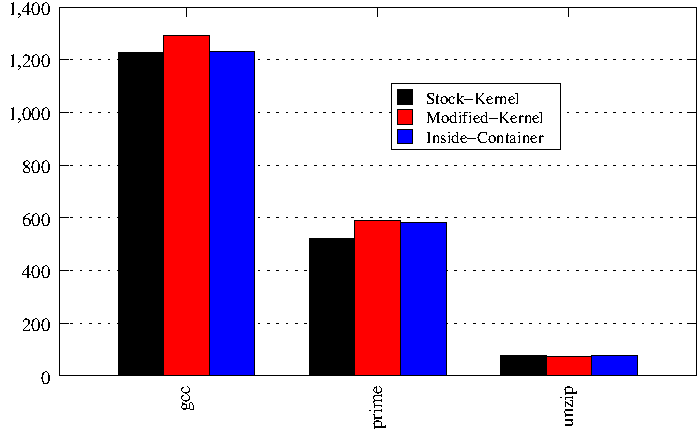
\includegraphics[width=1.0\columnwidth]{perf}
\caption{Running time comparison}
\label{fig:perf}
\end{figure}

%More detailed testing with LMbench3 (Section \ref{sec:LMbench3})proved that i/o, cpu, and memory performance were unaffected by the addition of the container code.  There was no overhead to running inside a container as well.  
\subsection{LXC Performance numbers}
In this section, we measure the overhead of our modifications to the kernel and the overhead due to running processes inside a container. Figure \ref{fig:perf} plots the running time of the following applications:
\begin{itemize}
    \item Compiling apache server
    \item Finding prime numbers between 0 and 500,000
    \item Unzipping a 200MB file.
\end{itemize}
From the figure, we can see that the overhead is approximately within 5\%-10\% and that running a process within a container does not significantly increase the running time.

%Our addition of the linux container functionality to the kernel imposed no noticeable overhead to the phone.  Our testing (Figure \ref{fig:perf}) proved that both the container kernel as well as the containers themselves, added no overhead to execution times.  

\begin{figure}[tbh]
\centering
\includegraphics[width=1.0\columnwidth]{quake}
\caption{Execution Time for the Quake time-demo}
\label{fig:Quake}
\end{figure}

\subsection{Quake Time-Demo}
\label{sec:quake_demo}
To measure the overhead of communicating from the container to an X-server running natively, we run the Quake timedemo \Comment{need ref}. The quake binaries were obtained from a Palm Pre port of the libsdl.org implementation and the command used to run the experiments was "quake +timedemo demo2". Figure \ref{fig:Quake} presents the running time of the demo in different scenarios. From the graph, we can see that the running time is similar for the stock kernel and the modified kernel. When the experiment is run from within the container, we observe that the running time increases by about 60\%. We attribute this to the fact that the containers are configured to create a new namespace for IPC and hence the application communicates with the X-Server through the loopback interface. When the containers are launched without a isolated IPC namespaces, we find that the performance is similar to that of the stock kernel.

\subsection{LMbench3} 
\label{sec:LMbench3}

\begin{figure*}[bth]
\centering
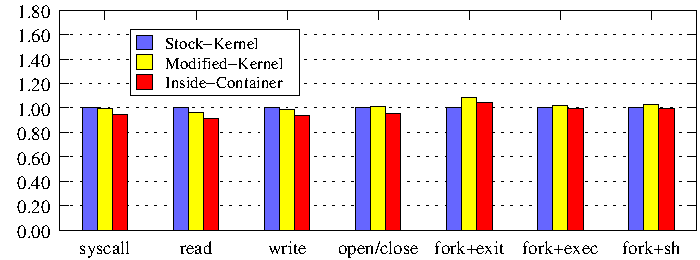
\includegraphics[width=2.0\columnwidth]{lmbench}
\caption{Normalized results from LMbench}
\label{fig:lmbench}
\end{figure*}

Our earlier experiments showed that there was no significant increase in the end-to-end running time of applications running inside a container.  We further run micro-benchmarks on the system in order to determine if there is any overhead pertaining to process creation, context switching, or creating files.

LMbench contains a suite of simple, portable benchmarks and is useful for comparing the performance of various UNIX systems.  It includes a variety of bandwidth benchmarks, of which the most popular are: cached file reads, memory operations (copy, read, and write), pipe, and TCP.  Additionally , it supports a wide variety of latency benchmarks, including: context switching, network connection establishment (pipe, TCP, UDP, RPC), file system operations (creates and deletes), process creation, handling of signals, system call overhead, and memory read latencies.  Lmbench also supports a variety of multiprocessor tests and includes large databases of results to compare one's results to. \cite{lmbench_paper}. LMbench3 is the most mature and commonly used benchmark among the LMbench family.  It runs a wide variety of tests, ranging from intensive latency testing of cache misses to extensive context switching testing.  LMbench has been heavily used in industry as well as academia \cite{lmbench}.

Figures \ref{fig:lmbench} and \ref{fig:lmbench-files} present results from running LMbench on a modified kernel and from within a container, normalized to the time taken on a stock kernel.  From the results, we can see that the the overhead for system calls and for process creation are negligible compared to the stock kernel. We do not attribute any reason to read and write calls being faster in the modified kernel and believe this to be due to external noise. 
% variations 

\begin{figure*}[bth]
\centering
\includegraphics[width=2.0\columnwidth]{lmbench-files}
\caption{Normalized results from File System create/delete benchmarks in LMbench}
\label{fig:lmbench-files}
\end{figure*}

